\documentclass{beamer}
\setbeamertemplate{caption}[numbered]
\usepackage{multirow}
\usepackage{fancyhdr}
\usepackage{graphicx}
\usepackage{multimedia}

\usetheme{Berlin}  %{Berlin}{Hannover}{Singapore}{CambridgeUS}

\title{Generative Adversarial Networks for Automatic Image Colorization}
\subtitle{\textbf{Team}: Yet Another Layer - YAL}


\author{Cameron Fabbri, Md Jahidul Islam}

\begin{footnotesize}

\end{footnotesize}


\begin{document}
\date{}
%%%%%%%%%%%%%%%%%%%%%%%%%%%%%%%%%
\begin{frame}
\thispagestyle{empty}
\titlepage
\end{frame}
%%%%%%%%%%%%%%%%%%%%%%%%%%%%%%%%%

\section*{Introduction}
%%%%%%%%%%%%%%%%%
\begin{frame}
\frametitle{\textbf{Image Colorization}}

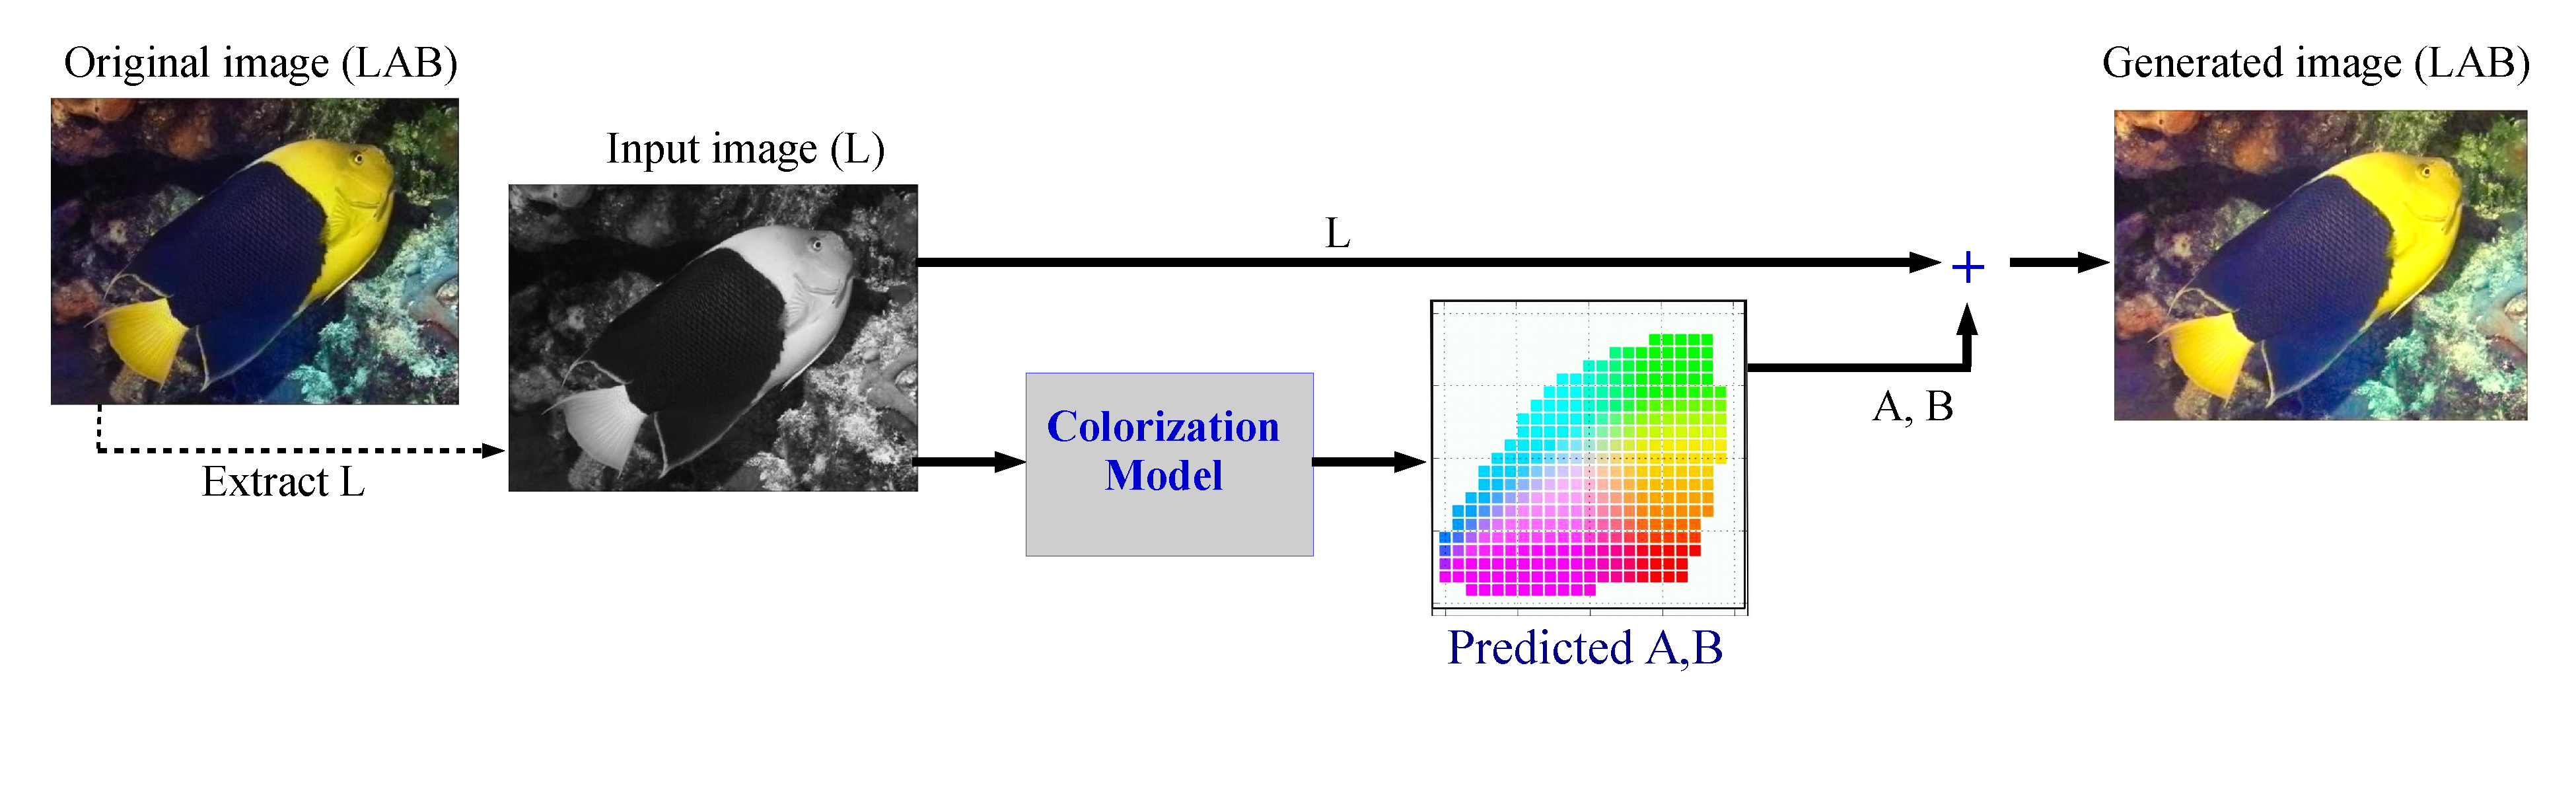
\includegraphics[width=\linewidth]{6.pdf}



\end{frame}
%%%%%%%%%%%%%%%%%%

\begin{frame}
\frametitle{\textbf{Background}}
\begin{itemize}
  \item Algorithmic choices:
	\begin{enumerate}[$-$]
	\item  \textbf{Image-to-image translation} 
	\item Classification
	\end{enumerate}
	
	\item Domain choices:
  
	\begin{enumerate}[$-$]
	\item  \textbf{LAB}, RGB
	\end{enumerate}
	
	\item Approaches
  
	\begin{enumerate}[$-$]
	\item Classical
	\item Deep learning based
	\begin{enumerate}[$-$]
	  \item Generative models
	  \item \textbf{Adversarial model}
	\end{enumerate}	 
	\end{enumerate}
	
\end{itemize}
\end{frame}
%%%%%%%%%%%%%%%%%%%%%%%


\section*{Background}

\section*{Classical and Generative Models}

\section*{GAN-based Models}

\section*{Results}



%\begin{frame}
%\begin{quote}
%\begin{center}
%\huge{Thank you all !} \\

%\end{center}   
%\end{quote}
%\end{frame}

\begin{frame}
\frametitle{\textbf{References}}
\footnotesize
\begin{enumerate}
\item Richard Zhang, Phillip Isola, and Alexei A Efros. Colorful image colorization. In European Conference on Computer Vision,
pages 649–666. Springer, 2016.
\item Huimin Lu, Yujie Li, and Seiichi Serikawa. Underwater image enhancement using guided trigonometric bilateral filter and fast
automatic color correction. In Image Processing (ICIP), 2013 20th IEEE International Conference on, pages 3412–3416. IEEE, 2013.
\item Luz A Torres-Méndez and Gregory Dudek. Color correction of underwater images for aquatic robot inspection. In International
Workshop on Energy Minimization Methods in Computer Vision and Pattern Recognition, pages 60–73. Springer, 2005.



\end{enumerate}
\end{frame}
\end{document}